\subsection{Introducci�n}
En esta secci�n se evaluan las pol��ticas de scheduling implementadas, utilizando diversas m�tricas especificadas m�s adelante.

\subsection{Ejercicio 6}
El objetivo de este ejercicio es programar un tipo de tarea \textbf{TaskBatch}, que durante \textit{total\_cpu} ciclos, realize \textit{cant\_bloqueos} llamadas bloqueantes, 
en momentos elegidos pseudoaleatoriamente. La implementaci�n consiste primero en precalcular todos los instantes en donde se van a realizar las
\textit{cant\_bloqueos} llamadas bloqueantes. Haciendo una analog�a con bolillas y urnas, si todos los posibles instantes entre el momento en que el proceso comienza a 
ejecutarse y el momento en que �ste termina de ejecutarse \textit{total\_cpu} ciclos despu�s, reprensentan las bolillas, lo que hacemos es elegir pseudoaleatoriamente
\textit{cant\_bloqueos} bolillas sin reposici�n, quedando asi determinados los momentos en los cuales se van a lanzar las llamadas bloqueantes. Luego, la tarea corre durante
\textit{total\_cpu} ciclos, utilizando la CPU o lanzando una llamada bloqueante seg�n corresponda.

Para m�s detalles, consultar la implementaci�n en \textit{tasks.cpp}.


\subsection{Ejercicio 7}

En este ejercicio debemos elegir 2 m�tricas diferentes y testear un lote de tareas \textbf{TaskBatch}, todas ellas con igual uso de CPU pero con diversas
cantidades de bloqueos. El lote de tareas utilizado es el \textit{lote3.tsk}.

Las m�tricas que elegimos fueron:
\begin{itemize}
 \item Turnaround
 \item Waiting Time 
\end{itemize}

Definidas en [Sil1] como:
\newline

\textbf{Turnaround}: Es el intervalo de tiempo entre el momento en que el proceso comienza a ejecutarse por primera vez, hasta el momento en que
el mismo termina. Es decir, es la suma de los per�odos usados en esperar datos de memoria, en estar encolado en la ``ready queue'', ejecutandose en 
la CPU, y haciendo E/S.


\textbf{Waiting Time}: Es el tiempo que un proceso se pasa encolado en la ``ready queue''.
\newline
\newline
Elegimos estas m�tricas ya que, con el Turnaround, tenemos una visi�n global de c�mo se comportan los procesos, mientras que con el Waiting Time
podemos observar c�mo un hecho m�s puntual, el tiempo que los procesos pasan encolados, impacta en el tiempo de ejecuci�n total del proceso.
\newline
\newline
Para calcular el desv�o standard utilizamos la f�rmula de [WikSD]
\newline
\newline
A continuaci�n se pueden observar los resultados de la experimentaci�n:
\newline
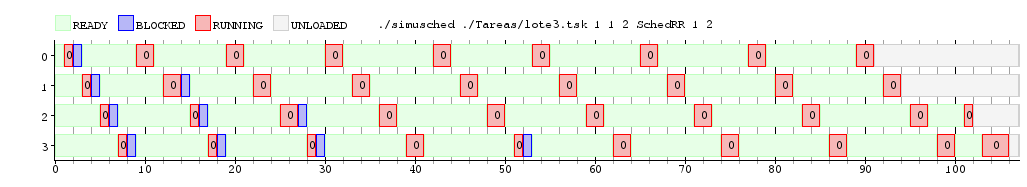
\includegraphics[width=1\textwidth]{./Graficos/ej7_1core_q2.png}
\begin{center}
 \textit{1 core, quantum = 2}.
\end{center}
~\\
\newline
Turnaround:  \hspace{7cm}  Waiting Time:

$P_{0}$: 90  \hspace{8cm}    $P_{0}$: 73

$P_{1}$: 91  \hspace{8cm}    $P_{1}$: 75

$P_{2}$: 97  \hspace{8cm}    $P_{2}$: 82

$P_{3}$: 99  \hspace{8cm}    $P_{3}$: 85


Promedio: 94,25 \hspace{6,5cm}   Promedio: 78,75


DS: 3,83         \hspace{7,7cm}    DS: 4,92
%----------------------------------------------------------------------------------------------

~\\
\newline
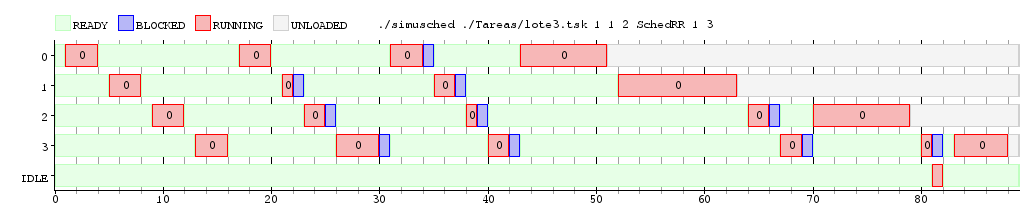
\includegraphics[width=1\textwidth]{./Graficos/ej7_1core_q3.png}
\begin{center}
 \textit{1 core, quantum = 3}.
\end{center}
~\\
\newline
Turnaround:  \hspace{7cm}  Waiting Time:

$P_{0}$: 81 \hspace{8cm}    $P_{0}$: 64

$P_{1}$: 82 \hspace{8cm}    $P_{1}$: 66

$P_{2}$: 90 \hspace{8cm}    $P_{2}$: 75

$P_{3}$: 91  \hspace{8cm}    $P_{3}$: 77


Promedio: 85,5  \hspace{6,5cm}    Promedio: 70,5


DS: 4,55        \hspace{7,6cm}    DS: 5,60
~\\
\newline


%----------------------------------------------------------------------------------------------

~\\
\newline
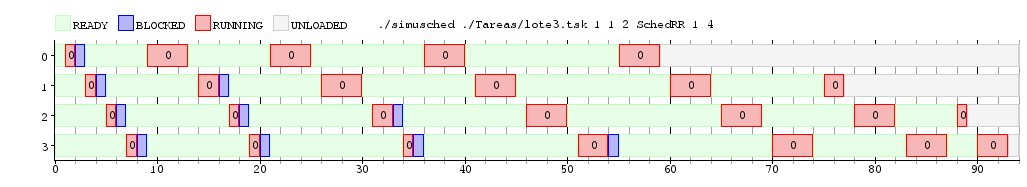
\includegraphics[width=1\textwidth]{./Graficos/ej7_1core_q4.png}
\begin{center}
 \textit{1 core, quantum = 4}.
\end{center}
~\\
\newline
Turnaround:  \hspace{7cm}  Waiting Time:

$P_{0}$: 58  \hspace{8cm}    $P_{0}$: 41

$P_{1}$: 74  \hspace{8cm}    $P_{1}$: 57

$P_{2}$: 84  \hspace{8cm}    $P_{2}$: 69

$P_{3}$: 86  \hspace{8cm}    $P_{3}$: 72


Promedio: 75,5   \hspace{6,7cm}    Promedio: 59,75


DS: 10,33         \hspace{7,5cm}    DS: 12,19
~\\
\newline




%----------------------------------------------------------------------------------------------

~\\
\newpage
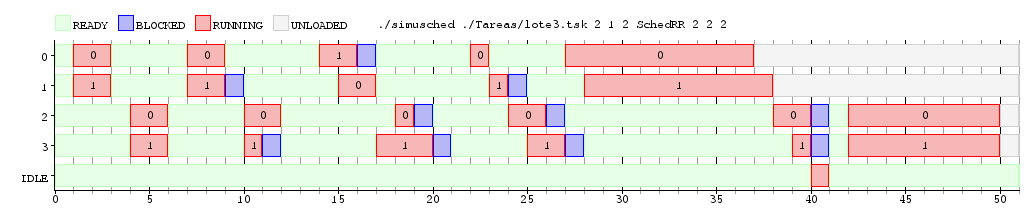
\includegraphics[width=1\textwidth]{./Graficos/ej7_2core_q2.png}
\begin{center}
 \textit{2 core, quantum = 2}.
\end{center}
~\\
\newline
Turnaround:  \hspace{7cm}  Waiting Time:

$P_{0}$: 47  \hspace{8cm}    $P_{0}$: 30

$P_{1}$: 49  \hspace{8cm}    $P_{1}$: 31

$P_{2}$: 51  \hspace{8cm}    $P_{2}$: 50

$P_{3}$: 51  \hspace{8cm}    $P_{3}$: 33


Promedio: 49,5 \hspace{6,6cm}    Promedio: 36


DS: 1,66       \hspace{7,6cm}    DS: 8,15
~\\
\newline




%----------------------------------------------------------------------------------------------

~\\
\newline
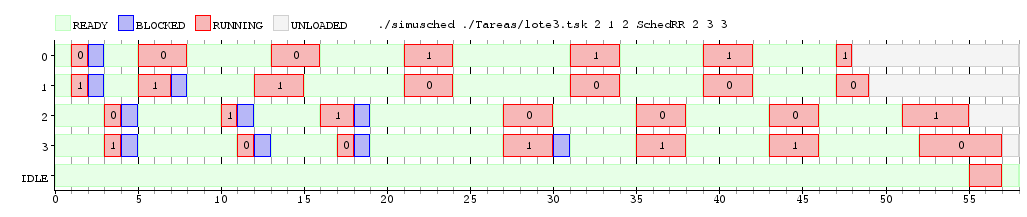
\includegraphics[width=1\textwidth]{./Graficos/ej7_2core_q3.png}
\begin{center}
 \textit{2 core, quantum = 3}.
\end{center}
~\\
\newline
Turnaround:  \hspace{7cm}  Waiting Time:

$P_{0}$: 47  \hspace{8cm}    $P_{0}$: 30

$P_{1}$: 48  \hspace{8cm}    $P_{1}$: 30

$P_{2}$: 52  \hspace{8cm}    $P_{2}$: 35

$P_{3}$: 54  \hspace{8cm}    $P_{3}$: 36


Promedio: 50,25  \hspace{6,4cm}    Promedio: 32,75


DS: 2,86         \hspace{7,6cm}    DS: 2,77
~\\
\newline




%----------------------------------------------------------------------------------------------

~\\
\newpage
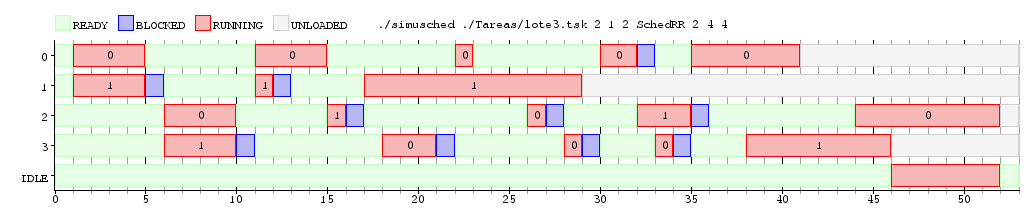
\includegraphics[width=1\textwidth]{./Graficos/ej7_2core_q4.png}
\begin{center}
 \textit{2 core, quantum = 4}.
\end{center}
~\\
\newline
Turnaround:  \hspace{7cm}  Waiting Time:

$P_{0}$: 35  \hspace{8cm}    $P_{0}$: 18

$P_{1}$: 45  \hspace{8cm}    $P_{1}$: 27

$P_{2}$: 48  \hspace{8cm}    $P_{2}$: 31

$P_{3}$: 53  \hspace{8cm}    $P_{3}$: 35


Promedio: 45,25  \hspace{6,5cm}    Promedio: 27,75


DS: 6,57        \hspace{7,6cm}    DS: 6,30
~\\
\newline


%----------------------------------------------------------------------------------------------

~\\
\newline
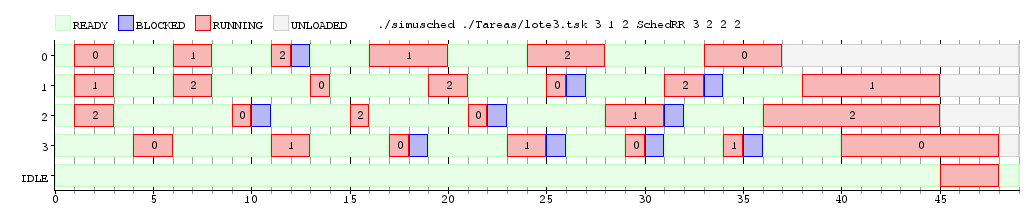
\includegraphics[width=1\textwidth]{./Graficos/ej7_3core_q2.png}
\begin{center}
 \textit{3 core, quantum = 2}.
\end{center}
~\\
\newline
Turnaround:  \hspace{7cm}  Waiting Time:

$P_{0}$: 43  \hspace{8cm}    $P_{0}$: 26

$P_{1}$: 47  \hspace{8cm}    $P_{1}$: 29

$P_{2}$: 49  \hspace{8cm}    $P_{2}$: 30

$P_{3}$: 49  \hspace{8cm}    $P_{3}$: 31


Promedio: 47  \hspace{6,9cm}    Promedio: 29


DS: 2,45          \hspace{7,6cm}    DS: 1,87
~\\
\newline



%----------------------------------------------------------------------------------------------

~\\
\newpage
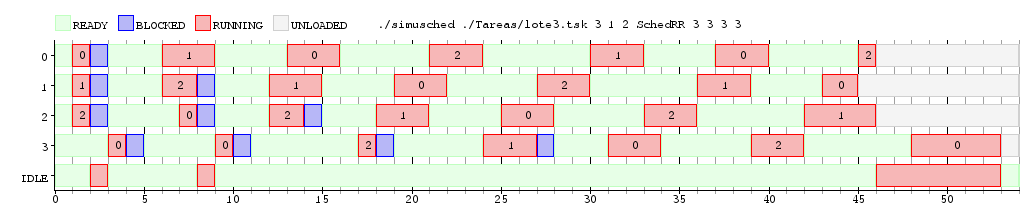
\includegraphics[width=1\textwidth]{./Graficos/ej7_3core_q3.png}
\begin{center}
 \textit{3 core, quantum = 3}.
\end{center}
~\\
\newline
Turnaround:  \hspace{7cm}  Waiting Time:

$P_{0}$: 45  \hspace{8cm}    $P_{0}$: 28

$P_{1}$: 44  \hspace{8cm}    $P_{1}$: 26

$P_{2}$: 45  \hspace{8cm}    $P_{2}$: 26

$P_{3}$: 50  \hspace{8cm}    $P_{3}$: 32


Promedio: 46   \hspace{6,9cm}    Promedio: 28


DS: 2,34        \hspace{7,6cm}    DS: 2,45
~\\
\newline



%----------------------------------------------------------------------------------------------

~\\
\newline
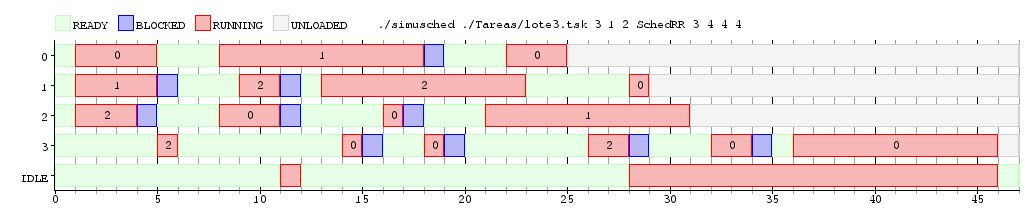
\includegraphics[width=1\textwidth]{./Graficos/ej7_3core_q4.png}
\begin{center}
 \textit{3 core, quantum = 4}.
\end{center}
~\\
\newline
Turnaround:  \hspace{7cm}  Waiting Time:

$P_{0}$: 28  \hspace{8cm}    $P_{0}$: 11

$P_{1}$: 35  \hspace{8cm}    $P_{1}$: 17

$P_{2}$: 36  \hspace{8cm}    $P_{2}$: 17

$P_{3}$: 39  \hspace{8cm}    $P_{3}$: 21


Promedio: 34,5  \hspace{6,6cm}    Promedio: 16,5


DS: 4,03          \hspace{7,6cm}    DS: 3,57 
~\\
\newline


Las conclusiones que pudimos sacar fueron las siguientes:

\begin{itemize}
 \item Dada una cantidad $i$ de cores, a medida que se aumenta el quantum, el tiempo promedio de Turnaround y Waiting Time disminuye. Esto en principio
 indicar�a que es buena idea aumentar el quantum, pero sin embargo a medida que se aumenta este, aumenta tambi�n el desv�o est�ndar, lo cual implica que los valores
 de Turnaround y Waiting Time se encuentran m�s dispersos. Esto significa que va a haber procesos que terminen relativamente r�pido mientras que otros no, lo cual disminuye
 el \textit{fairness} del sistema.
 \item Dado un mismo valor de quantum, aumentar la cantidad de cores siempre disminuye el tiempo promedio de Turnaround y Waiting Time, manteniendo o 
 reduciendo a su vez el desv�o est�ndar. Por lo tanto, obviamente, un aumento en la cantidad de cores siempre es beneficioso.
 \item El Waiting Time representa una parte muy importante del Turnaround: aproximadamente un 81\% en el caso de 1 core, 65\% con 2 cores, y 53\% con 3 cores.
 \item L�gicamente, los procesos que m�s llamadas bloqueantes realizan son los que m�s tiempo tardan en terminar. Sin embargo, en la mayor parte de los casos, 
 la diferencia en los valores de Turnaround no es demasiado significativa.
 \item El valor �ptimo del quantum para ambas m�tricas ser�a $4$, si se tolera el desv�o est�ndar asociado.
\end{itemize}


\subsection{Ejercicio 8}
En la presente secci�n vamos a trabajar sobre un algoritmo de scheduling de tipo Round Robin pero que no permite la migraci�n de procesos entre
n�cleos. Para tal motivo se utiliza una cola de \texttt{READY} para cada core, donde una vez que el proceso llega se moviliza s�lo por esa cola.

Cuando el proceso es bloqueado debemos tener una manera de saber a qu� CPU pertenec�a dicho proceso, y para tal fin cada core tambi�n tiene una
cola de \texttt{BLOQUED}. Entonces, cuando un proceso es desbloqueado simplemente se lo busca en alguna de las listas \texttt{BLOQUED} de los cores,
y una vez que se lo encuentra se lo agrega a la cola \texttt{READY} correspondiente al core que ten�a esa tarea bloqueada. Esto hace que cada CPU
tenga un esquema de Round Robin de un s�lo core independiente del resto.

A continuaci�n mostramos un gr�fico correspondiente al procesamiento del lote de tareas \textit{lote5.tsk} para este nuevo scheduler.
Las tareas se encolan acorde a su momento de llegada y a la carga de los dem�s cores. Las tres primeras se cargan una en cada core, la cuarta
se carga en el primer core ya que todos estan igualmente cargados. Luego todas siguen ejecut�ndose en sus respectivos cores sin cambios de
lugar como es esperado.


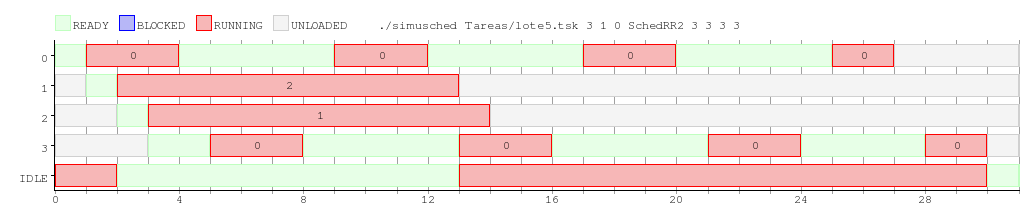
\includegraphics[width=1\textwidth]{./Graficos/ej8_1.png}
\begin{center}
 \textit{Cores = 3, Qantum = 3 cada core, CS = 1}.
\end{center}

Ahora, con el objetivo de comparar con la pol�tica de scheduling de una sola cola, vamos a correr el mismo lote para ver c�mo se comporta.
A continuaci�n se encuentra el gr�fico con la distribuci�n de las tareas.

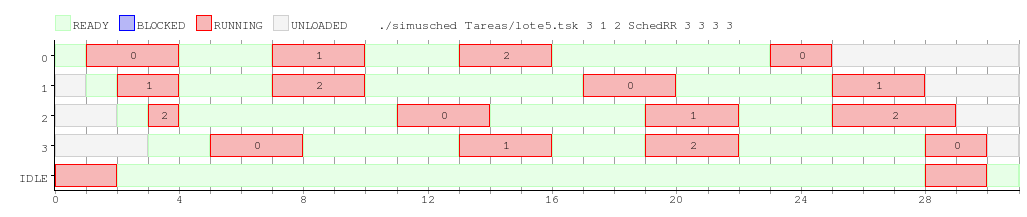
\includegraphics[width=1\textwidth]{./Graficos/ej8_2.png}
\begin{center}
 \textit{Cores = 3, Qantum = 3 cada core, CS = 1, CI = 2}.
\end{center}

Un detalle que vale la pena mencionar es que las tareas desde que iniciar hasta que finalizar estan asociadas a un solo core en el caso del
grafico uno. No ocurre asi en el gr�fico 2, en donde porciones de la tarea van cambiando de core, como se ve en el segundo gr�fico.

Para este lote de tareas en particular podemos apreciar que \texttt{SchedRR2} y \texttt{SchedRR} finalizan la ejecuci�n de todas las tareas
en un tiempo similar. Pero en el primer caso dos de las tareas finalizan r�pido, algo que no sucede en el segundo caso, sin contar que en
\texttt{SchedRR2} no hay costos por cambio de core, que s� presenta \texttt{SchedRR}.

Por otro lado, si bien es cierto que \texttt{SchedRR2} termina dos de las tres tareas m�s r�pido, tambi�n es cierto que esos cores quedan
inactivos el resto del tiempo (para este lote) algo que no es deseable. Esta comparativa nos brinda un indicio de que si bien \texttt{SchedRR2}
parece m�s eficiente, para algunos escenarios puede presentar desventajas con respecto a \texttt{SchedRR}, y dicho escenario es cuando
un core se queda con muchas tareas pendientes y los dem�s no poseen ninguna. Para estos casos se podr�a implementar alguna pol�tica de balance
de carga, es decir, si un core tiene muchas tareas y los dem�s ninguna, se podr�an mover algunas tareas del core m�s ocupado para los de menos
carga. En este caso estar�amos pagando la penalizaci�n del cambio de core (por el traslado de colas), pero es preferible eso antes que alg�n
core quede inactivo.

A continuaci�n vamos a correr nuevamente los dos schedulers con el lote de tareas \texttt{lote6.tsk} que resultar� en tareas pesadas para
el core 0, y tareas mas livianas para el resto. El primer core tendr� un quantum mas grande que los otros. La idea es mostrar un escenario
en donde puedo aprovechar cierta caracter�stica de los cores.

La idea detr�s del dise�o de este lote es construirlo para que el core 0 tome las tareas mas pesadas (en cuanto a CPU) y el resto las m�s
livianas. Adem�s se configura la corrida del scheduler con tres cores, de los cuales el primero tiene un quantum mas alto que los dem�s.
As� queda el procesamiento del \texttt{lote6.tsk} con \texttt{SchedRR2}:

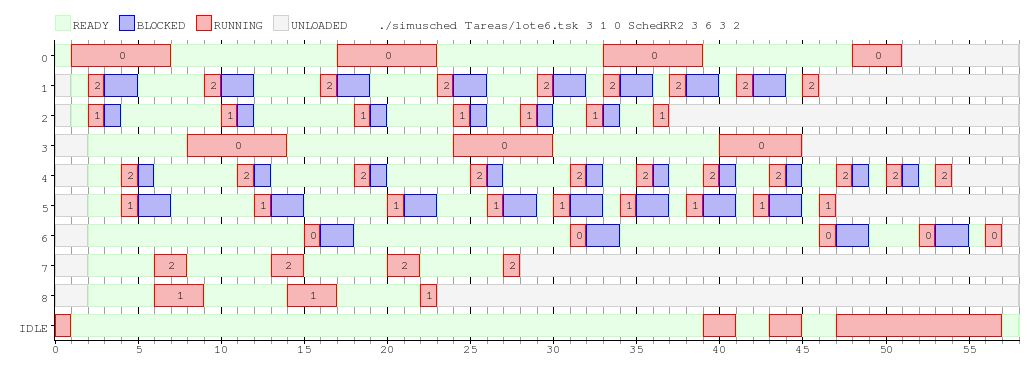
\includegraphics[width=1\textwidth]{./Graficos/ej8_3.png}
\begin{center}
 \textit{Cores = 3, Qantum = 3 cada core, CS = 1}.
\end{center}

Y con \texttt{SchedRR} el procesamiento de dicho lote queda de la siguiente forma:

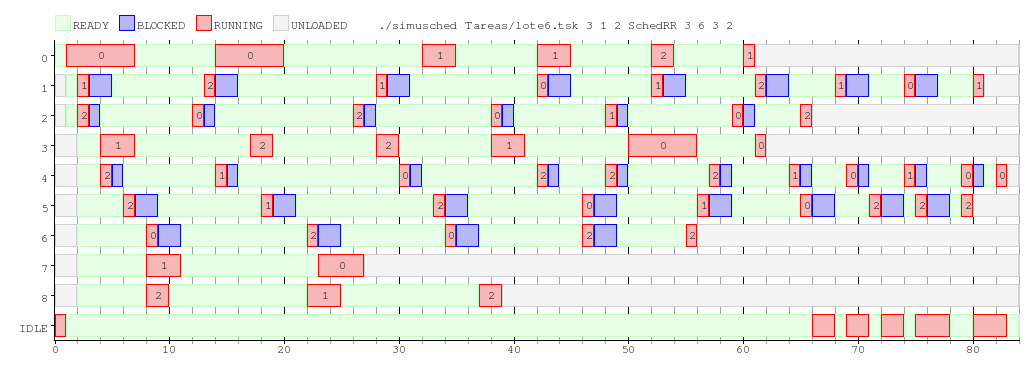
\includegraphics[width=1\textwidth]{./Graficos/ej8_4.png}
\begin{center}
 \textit{Cores = 3, Qantum = 3 cada core, CS = 1, CI = 2}.
\end{center}

Vemos que para este lote, \texttt{SchedRR2} tiene mejor performance. Las tareas son finalizadas m�s r�pido, y todo el lote es procesado
m�s r�pido que en \texttt{SchedRR}. A�n as� en \texttt{SchedRR2} tenemos bastante tiempo de procesamiento en donde un procesador u otro permanece ocioso.
Eso ocurre tambi�n en \texttt{SchedRR} pero es menor la cantidad de tiempo que los cores permanecen ociosos, aunque el desempe�o final es peor.

\section{Ejercicio 9}
En esta parte del trabajo vamos a analizar la \textit{fairness} del algoritmo de scheduling
\texttt{SchedLottery}. Tomamos como definici�n de \textit{fairness} al hecho de que cada
proceso reciba igual cantidad de tiempo de CPU, o m�s precisamente, un tiempo apropiado para
cada proceso de acuerdo a su prioridad y carga de trabajo.

A continuaci�n vamos a mostrar los experimentos realizados para poder ver que efectivamente
cuando se realizan \textit{n} experimentos, el scheduler es realmente justo cuando \textit{n} aumenta su tama�o.
Notar que es necesario hacer m�s de una corrida ya que debido al factor pseudoaleatorio del
algoritmo, realizar una o dos corridas no es suficiente para ver que efectivamente el scheduler
es justo.


\subsection{Ejercicio 10}

Dadas las implementaciones de $ShedLottery$, con o sin tickets compensatorios (respectivamente en $sched\_lottery.cpp$ y $sched\_lottery\_base.cpp$), el ejercicio nos propone ponerlas a prueba y compararlas, relacion\'andolas con la problem\'atica que presentaban los autores y verificar si los tickets compensatorios son una soluci\'on viable. 

\vspace{2mm}

Para esto generamos dos lotes distintos: \textbf{Lote7}, que consta de 3 tareas intensivas de CPU y una tarea de I/O bloqueante, y para comprobar que el mecanismo funciona con varias tareas bloqueadas al mismo tiempo, el lote \textbf{Lote8} con 2 tareas intenstivas de CPU y 2 bloqueantes.

\vspace{2mm}
\textbf{Lote7:}

\begin{lstlisting}[numbers=none]
@0:
*3 TaskCPU 50
*1 TaskConsola 50 1 2
\end{lstlisting}

\vspace{2mm}
\textbf{Lote8:}

\begin{lstlisting}[numbers=none]
@0:
*2 TaskCPU 50
*2 TaskConsola 25 1 2
\end{lstlisting}

\subsubsection{Experimentos: Lote 7}

\vspace{2mm}

Los experimentos fueron realizados con los par\'ametros: \textbf{semilla} aleatoria(pero la misma para cada comparaci\'on entre schedulers), \textbf{quantum} de tres ticks, \textbf{bloqueos} de un tick (con el objetivo de generar muchos cambios de contexto y tener m\'as casos de an\'alisis), \textbf{cantidad de procesadores} de uno y costo de \textbf{cambio de contexto} de cero, para hacer m\'as sencillo el an\'alisis y no agregar variables que no aportan al experimento.

\vspace{2mm}

\textbf{Caso1:}

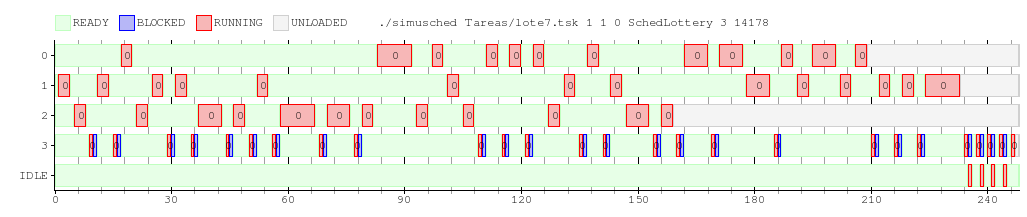
\includegraphics[width=1\textwidth]{./Graficos/Ej10v2/Task7/ej9_1.png}
\begin{center}
 \textit{Scheduler = Compensatorio, Semilla = 14178}.
\end{center}


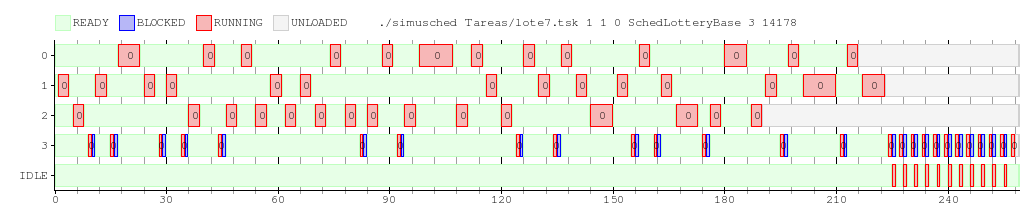
\includegraphics[width=1\textwidth]{./Graficos/Ej10v2/Task7/ej9_1_base.png}
\begin{center}
 \textit{Scheduler = No Compensatorio, Semilla = 14178}.
\end{center}

\vspace{2mm}


Pueden notarse las 3 tareas intensivas de CPU y la tarea I/O, que procesa 1 tick y se bloquea. Aqui vemos como, en el caso sin compensation tickets, la tarea se bloquea, perdiendo $2/3$ de su quantum y luego vuelve a obtener el cpu muchos ticks despues, perdiendo tiempo de procesamiento. Esto se nota claramente al ver que m\'as de la mitad de su tiempo de procesamiento se produce al final de la simulaci\'on.

\vspace{2mm}

En el caso con compensation tickets, puede notarse como luego de bloquearse, en el siguiente cambio de contexto a su desbloqueo vuelve a obtener la cpu en varios casos, producto de su aumento de probabilidad gracias a los compensation tickets. Pueden compararse adem\'as ambos finales de las simulaciones y notar que, en la simulaci\'on con tickets compensatorios, restan muchos menos ticks de la tarea I/O por procesar.

\vspace{2mm}
\textbf{Caso2:}

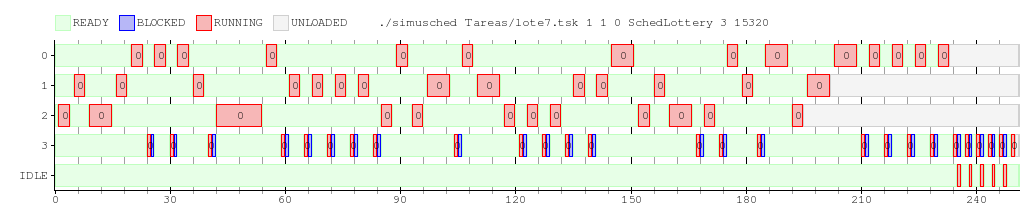
\includegraphics[width=1\textwidth]{./Graficos/Ej10v2/Task7/ej9_2.png}
\begin{center}
 \textit{Scheduler = Compensatorio, Semilla = 15320}.
\end{center}


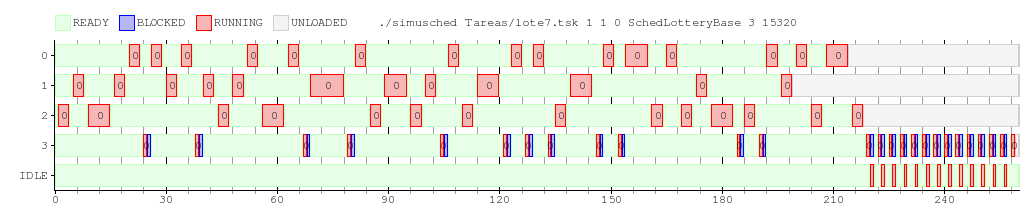
\includegraphics[width=1\textwidth]{./Graficos/Ej10v2/Task7/ej9_2_base.png}
\begin{center}
 \textit{Scheduler = No Compensatorio, Semilla = 15320}.
\end{center}

En este caso pueden observarse tambi\'en bursts de la tarea I/O, y puede notarse adem\'as que una vez que la tarea pierde la asignaci\'on de la CPU en su tick compensado, es poco probable que la vuelva a obtener por un per\'iodo, ya que debido a la implementaci\'on de tickets compensatorios, si una tarea compensada pierde la asignac\'on, sus tickets compensatorios son retirados de todas formas.

\vspace{2mm}
\textbf{Caso3:}


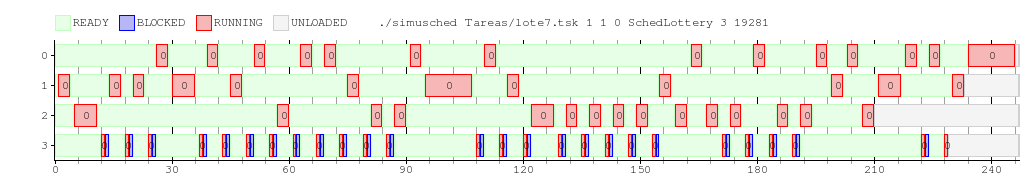
\includegraphics[width=1\textwidth]{./Graficos/Ej10v2/Task7/ej9_3.png}
\begin{center}
 \textit{Scheduler = Compensatorio, Semilla = 19281}.
\end{center}


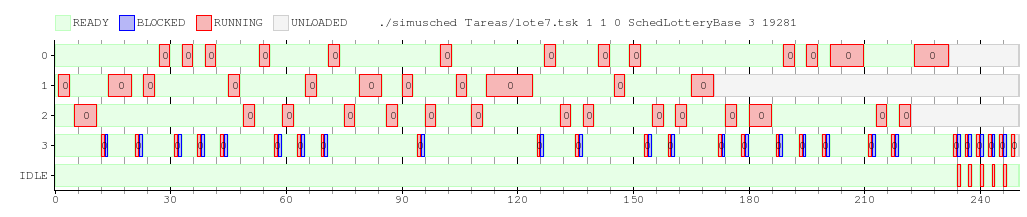
\includegraphics[width=1\textwidth]{./Graficos/Ej10v2/Task7/ej9_3_base.png}
\begin{center}
 \textit{Scheduler = No Compensatorio, Semilla = 19281}.
\end{center}

En este caso se aprecia claramente que la implementaci\'on de tickets compensatorios equilibra efectivamente la asignaci\'on de CPU, ya que comparado con la simulaci\'on no compensada, donde la tarea I/O debe terminar su ejecuci\'on al \'ultimo, en el caso compensado esta tarea recibe la asignaci\'on del CPU mucho m\'as frecuentemente, e incluso finaliza su ejecuci\'on \textbf{antes} que dos de las dem\'as.

\vspace{2mm}
\textbf{Caso4:}


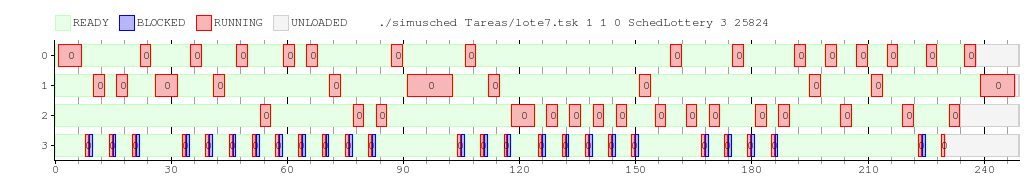
\includegraphics[width=1\textwidth]{./Graficos/Ej10v2/Task7/ej9_4.png}
\begin{center}
 \textit{Scheduler = Compensatorio, Semilla = 25824}.
\end{center}


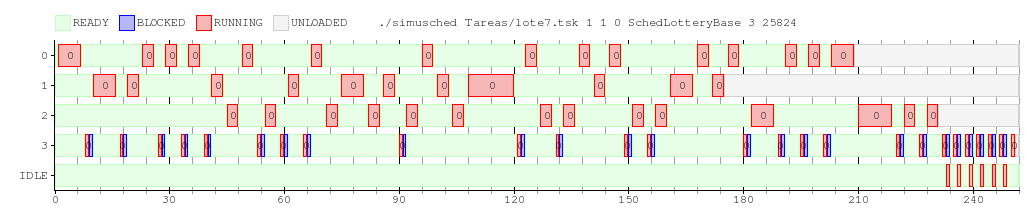
\includegraphics[width=1\textwidth]{./Graficos/Ej10v2/Task7/ej9_4_base.png}
\begin{center}
 \textit{Scheduler = No Compensatorio, Semilla = 25824}.
\end{center}

El \'ultimo caso analizado refleja correctamente todo lo anteriormente planteado. De esta forma concluimos en que en el caso de una tarea que se bloquea frecuentemente y compite por el CPU contra varias otras de uso intensivo de \'este, la implementaci\'on de tickets compensatorios logra homogeneizar la asignaci\'on y aprovechar ciclos de procesamiento.

\subsubsection{Experimentos: Lote 8}

\vspace{2mm}

Con el lote 8 analizamos si el mecanismo se mantiene eficiente cuando hay m\'as de una tarea I/O en ejecuci\'on.

\vspace{2mm}


\textbf{Caso1:}

\vspace{2mm}

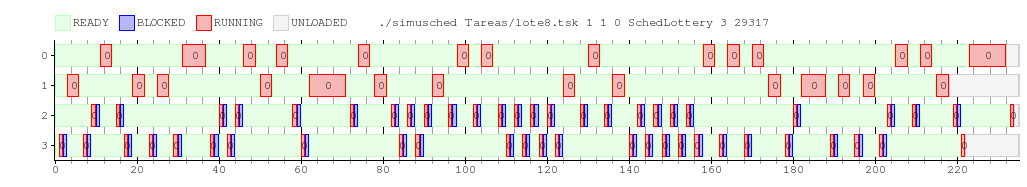
\includegraphics[width=1\textwidth]{./Graficos/Ej10v2/Task8/ej9_3.png}
\begin{center}
 \textit{Scheduler = Compensatorio, Semilla = 29317}.
\end{center}


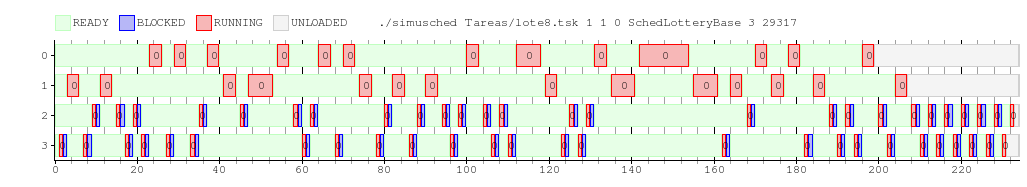
\includegraphics[width=1\textwidth]{./Graficos/Ej10v2/Task8/ej9_3_base.png}
\begin{center}
 \textit{Scheduler = No Compensatorio, Semilla = 29317}.
\end{center}

\vspace{2mm}

A primera vista puede notarse que el mecanismo contin\'ua siendo eficiente, ya que en el modo compensado las tareas I/O terminan junto con las dem\'as, en cambio en el modo no compensado finalizan \'ultimas.
\vspace{2mm}

\textbf{Caso2:}

\vspace{2mm}

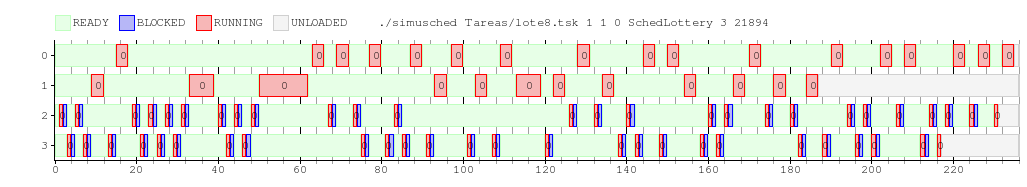
\includegraphics[width=1\textwidth]{./Graficos/Ej10v2/Task8/ej9_4.png}
\begin{center}
 \textit{Scheduler = Compensatorio, Semilla = 21894}.
\end{center}


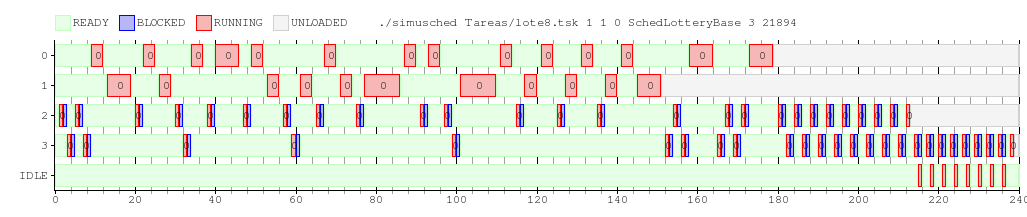
\includegraphics[width=1\textwidth]{./Graficos/Ej10v2/Task8/ej9_4_base.png}
\begin{center}
 \textit{Scheduler = No Compensatorio, Semilla = 21894}.
\end{center}

\vspace{2mm}


En este caso es a\'un m\'as notoria la tendencia, ya que en el modo no compensado las tareas I/O poseen casi todo su tiempo de procesamiento al final, en cambio en el modo compensado todas las tareas finalizan aproximadamente al mismo momento. Puede apreciarse como se aprovechan ticks de CPU, simplemente con ver la escala de ticks. Esto muestra que es eficiente priorizar la asignaci\'on de CPU a las tareas que se bloquean constantemente, ya que consumen poco tiempo de CPU y vuelven a bloquearse, trasfiriendo la CPU a otras tareas. De otra forma son relegadas hasta el final de la ejecuci\'on, y en sus bloqueos ya no quedan tareas y se debe switchear a la tarea IDLE.

\vspace{2mm}

\textbf{Caso3:}

\vspace{2mm}

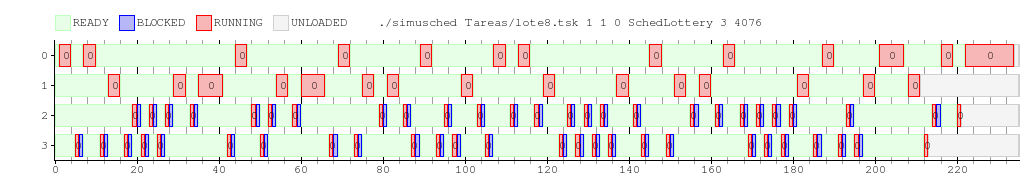
\includegraphics[width=1\textwidth]{./Graficos/Ej10v2/Task8/ej9_5.png}
\begin{center}
 \textit{Scheduler = Compensatorio, Semilla = 4076}.
\end{center}


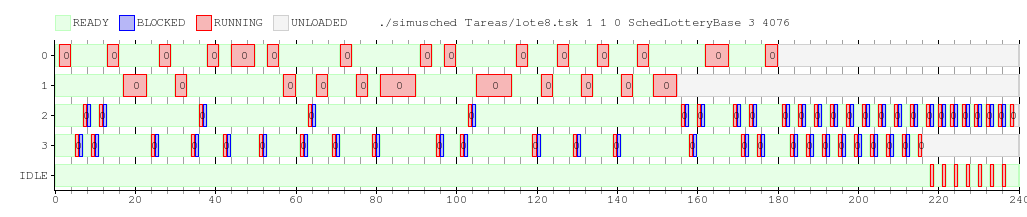
\includegraphics[width=1\textwidth]{./Graficos/Ej10v2/Task8/ej9_5_base.png}
\begin{center}
 \textit{Scheduler = No Compensatorio, Semilla = 4076}.
\end{center}

\vspace{2mm}

Con este caso finalizamos el an\'alisis. ya que consideramos que los resultados son claros y que el mecanismo de compensation tickets, tal como lo describen los autores es muy efectivo en solucionar la problem\'atica de la asignaci\'on justa del CPU para aquellas tareas que se bloquean y no consumen su quantum entero. Mediante los compensation tickets, no s\'olo se vuelve m\'as justa la asignaci\'on, sino que tambi\'en se aprovechan ticks de procesamiento.
